\documentclass[a4paper,10pt]{article}
\usepackage[utf8]{inputenc}
\usepackage{amsthm}
\usepackage{amssymb}
\usepackage[T1]{fontenc}
\usepackage{babel}

\setlength{\parskip}{8pt} % space between paragraphs

\usepackage{float}%H dans figure
\usepackage{bm}% lettre math gras et italique -> remplace \v v
\usepackage{tabularx}
\usepackage[modulo,mathlines]{lineno}
\usepackage{xfrac} %\sfrac
\usepackage{tikz}
\usepackage{textcomp}
\usetikzlibrary{arrows,shapes}
\usepackage{etoolbox}
\usetikzlibrary{patterns}
\usetikzlibrary{calc}
\usetikzlibrary{arrows}
\usepackage[hang,small]{caption}
\usetikzlibrary{patterns}
\usepackage{calc}

\usetikzlibrary{calc}
\usepackage{amsmath}
\usepackage{array}
\usepackage{delarray}
\usepackage{multicol}
\usepackage{subcaption}

\usepackage{ifthen}
\usepackage{algorithm}
\usepackage{algpseudocode}
\usepackage[margin=0.25in]{geometry}

\usepackage{pgfplots}
\pgfplotsset{width=10cm,compat=1.9}
\usetikzlibrary{arrows.meta,calc,decorations.pathreplacing,positioning}
\newcommand{\bnabla}{\bm{\nabla}}
\newcommand{\bsigma}{\bm{\sigma}}
\newcommand{\bv}{\bm{v}}
\newcommand{\manualindent}{\hspace{2em}}

\newcommand{\ep}{\varepsilon}
\newcommand{\be}{\begin{equation}}
\newcommand{\ee}{\end{equation}}
\newcommand{\ba}{\begin{array}}
\newcommand{\ea}{\end{array}}
\newcommand{\bc}{\begin{cases}}
\newcommand{\ec}{\end{cases}}
\newcommand{\norm}[1]{\left\lVert#1\right\rVert}

\newcommand{\bs}{\begin{split}}
\newcommand{\es}{\end{split}}

\newcommand{\bsc}{
	\left\{
	\begin{array}{l}
}
\newcommand{\esc}{
	\end{array}\right.
}
\newcommand{\dis}{\displaystyle}

%% definition des marges
\topmargin = -10mm
\oddsidemargin = 0mm
\evensidemargin = 0mm
\setlength{\textwidth}{16cm}
\setlength{\textheight}{24cm}


\colorlet{myblue}{green!30!blue}
\colorlet{mygreen}{blue!30!green}
\definecolor{alizarin}{rgb}{0.82, 0.1, 0.26}
\definecolor{amber}{rgb}{1.0, 0.75, 0.0}
\definecolor{amethyst}{rgb}{0.6, 0.4, 0.8}
\definecolor{ballblue}{rgb}{0.13, 0.67, 0.8}
\definecolor{cadetblue}{rgb}{0.37, 0.62, 0.63}
\definecolor{cadmiumred}{rgb}{0.89, 0.0, 0.13}
\definecolor{candyapplered}{rgb}{1.0, 0.03, 0.0}
\definecolor{caribbeangreen}{rgb}{0.0, 0.8, 0.6}
\definecolor{carminered}{rgb}{1.0, 0.0, 0.22}
\definecolor{carnationpink}{rgb}{1.0, 0.65, 0.79}
\definecolor{celadon}{rgb}{0.67, 0.88, 0.69}
\definecolor{coral}{rgb}{1.0, 0.5, 0.31}
\definecolor{lavender}{rgb}{0.71, 0.49, 0.86}
\definecolor{lavenderrose}{rgb}{0.98, 0.63, 0.89}
\definecolor{neoncarrot}{rgb}{1.0, 0.64, 0.26}
\definecolor{unitednationsblue}{rgb}{0.36, 0.57, 0.9}
\definecolor{greentest}{rgb}{0.2, 0.8, 0.4}

\usepackage[colorlinks=true, linkcolor=myblue,citecolor=mygreen]{hyperref}
% \usepackage[colorlinks=false, linkbordercolor=red,citebordercolor=green, pdfborder={0 0 1}]{hyperref}

\setlength{\parindent}{0pt}
\setlength{\parskip}{1em}

\newtheorem{theorem}{Theorem}[section]
\newtheorem{prop}[theorem]{Proposition}
\newtheorem{Hyp}[theorem]{Assumption}
\newtheorem{lemma}[theorem]{Lemma}
\newtheorem{remark}[theorem]{Remark}
\newtheorem{definition}[theorem]{Definition}

\title{Finite Volume Method}
\author{LAINE Florian}
\date{May 2026}
\begin{document}
\maketitle
\tableofcontents

\section{Navier Stokes Equation}

Let $\bm{u}$ define the velocity vector and $\bm{p}$ define the pressure vector defined on $\Omega$.

\be
\bc
\nabla \cdot \bm{u} = 0 \\
\dis \frac{\partial \bm{u}}{\partial t} + (\bm{u} \cdot \nabla \bm{u}) \bm{u} + \frac{1}{\rho} \nabla \bm{p} - \nu \nabla^2 \bm{u} - \bm{g} = 0.
\ec
\label{navier_stokes}
\ee

\section{Discretisation}

We consider a mesh $\mathcal{M}$ over a surface $\Omega$ with polygons; along with the $\bm{x}$ spacial variable. Let $j$ be a polygonal cell of this mesh and $\ell$ an edge $[r, s]$. We will denote $\bm{n}_{\ell j}$ the outward from cell $j$ normal at the edge $\ell$. The centroid of the cell $j$ is $\bm{x}_j$, the middle of the edge $\ell$ is $\bm{x}_\ell$ and the position of the node of $r$ (resp. s) is called $\bm{x}_r$ (resp. $\bm{x}_s$). A second cell $k$ is said to be a neighbouring cell of $j$, if $\exists ! \ell \in \mathcal{M} : (\ell \in k) \cap (\ell \in j)$. The boudnaries of the 

\begin{figure}[H]
  \centering
	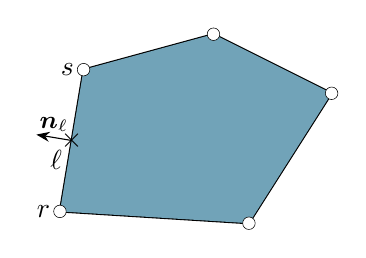
\begin{tikzpicture}[scale=1.5, solidnode/.style={circle,fill=black,inner sep=1.6pt},opencircle/.style={circle,draw=black,very thin,inner sep=1.6pt}, bar/.style={line width=0.7pt,draw=black},arrowstyle/.style={-Stealth,thin}]

 \coordinate (a) at (0.5,0.5);
 \coordinate (b) at (0.7,1.7);
 \coordinate (c) at (1.8,2);
 \coordinate (d) at (2.8,1.5);
 \coordinate (e) at (2.1,0.4);

 \coordinate (ell) at ($(a)!0.5!(b)$);

    \draw[thick] (a) -- (b) -- (c) -- (d) -- (e) -- cycle;
    \fill[color=cyan!40!gray] (a) -- (b) -- (c) -- (d) -- (e) -- cycle;
\foreach \p in {a,b,c,d, e}
			\node[opencircle, fill=white] at (\p) {};

	\draw (a) node [left] {$r$};
	\draw (b) node [left] {$s$};

	\draw (ell) node [below left] {$\ell$};
	\draw (ell) node [] {$\times$};
  \coordinate (nell) at ($ (ell)!0.5!90:(b) $);
  \draw [arrowstyle](ell)--(nell) node [above right,inner sep=1pt] {\small $\bm{n}_{\ell}$};
\end{tikzpicture}
\caption{A cell $j$, an edge $\ell$ and its normal $\bm{n}_\ell$}
  \label{fig:example_cell}
\end{figure}
We start by recalling divergence theorem. Given a field $\bm{u}$ and a closed surface $V$,
\be
\int_V \nabla \cdot \bm{u}\, dV = \int_{\partial V} \bm{n} \cdot \bm{u} \, dS
\label{divergence_theorem}
\ee
where $\partial V$ denotes the boundaries of the closed surface $V$ and $\bm{n}$ the outpointing normal.

We define the field $\bm{u}^\star$, so that
\be
\dis \frac{\partial \bm{u}^\star}{\partial t} + (\bm{u}^\star \cdot \nabla) \bm{u} - \nu \nabla^2 \bm{u}^\star - \bm{g} = 0.
\label{define_ustar}
\ee
which is, in essence, the same equation as \eqref{navier_stokes} but with the pressure field term omitted after applying a semi-implicit (resp. implicit) discretization of the and transport (resp. diffusion) term.

We will then integrate \eqref{define_ustar} over a cell $j$ (see figure \ref{fig:example_cell}) and discretize in time.
\be
\dis \int_j \frac{\bm{u}^\star - \bm{u}}{\Delta t} + (\bm{u}^\star \cdot \nabla) \bm{u} - \nu \nabla^2 \bm{u}^\star - \bm{g} = 0.
\label{integrate_ustar}

\ee
We now split this last equation and evalute term by term.

\subsection{Constant term}

\be
\int_j \bm{g} = V_j \bm{g}
\ee

\subsection{Convection term}
The convection term can be expressed using the divergence theorem \eqref{divergence_theorem},
\be
\dis \int_j (\bm{u}^\star \cdot \nabla) \bm{u} 
= \int_{\partial j} (\bm{u}^\star \cdot \bm{n}_{\partial j}) \bm{u}
= \sum_{\ell \in j} \int_\ell (\bm{u}^\star \cdot \bm{n}_{\ell j}) \bm{u}
= \sum_{\ell \in j} |\ell| (\bm{u}_\ell^\star \cdot \bm{n}_{\ell j}) \bm{u}_\ell.
\ee
Please 

% - \nu \nabla^2 \bm{u}^\star - \bm{g} = 0.


\end{document}

